\section*{Общая характеристика работы}

\paragraph {Актуальность темы и степень ее разработанности.}
Двустворчатый моллюск {\it Macoma balthica} (Linnaeus, 1758)~--- один из излюбленных модельных объектов в морских гидробиологических исследованиях. 
В классической биогеографии вид относят к амфибореальным. 
Это обычная литоральная форма в Белом море, у берегов Мурмана и далее на запад, вдоль атлантических берегов Европы~--- до Франции. 
По Атлантическому побережью Северной Америки макомы распространены от Лабрадора до штата Джорджия. 
В северной части Тихого океана~--- от Берингова моря до Японского, а по американскому побережью~--- до Калифорнии. 
В юго-восточной части Баренцева моря и в прилегающей части Карского моря они обитают  не на литорали, а на глубине нескольких метров. 
Моллюски заселяют всю основную часть Балтийского моря, далеко заходя во все заливы, где живут до глубины более 100 метров (\cite{Zacepin_Filatova_1968}).

В настоящее время вид {\it Macoma balthica} по результатам аллозимного анализа предлагают разделять на два подвида: {\it M.~b.~balthica}, обитающий в северной части Тихоокеанского региона, и {\it M.~b.~rubra} из Северо-Восточной Атлантики. 
Однако  в морях, связанных с  Атлантикой, существуют очаги распространения тихоокеанской формы. 
Так, в Балтийском и Баренцевом море Атлантическая и Тихоокеанская формы сосуществуют и образуют гибриды (\cite{Vainola_2003}). 
В Белом море встречается в основном {\it M.~b.~balthica}, и лишь в устье Онеги было обнаружено два экземпляра {\it M.~b.~rubra} (\cite{Nikula_et_al_2007}).
К настоящему моменту нет прямых данных о влиянии данных генетических особенностей на экологические характеристики особей, поэтому в данной работе рассматривается вид {\it Macoma balthica} sensu lato.


{\it Macoma balthica}~--- хорошо изученный вид в центральной части ареала (см. например: \cite{Segerstrale_1960, Lavoie_1970, Gilbert_1978, Vincent_et_al_1989, Hiddink_et_al_2002_predation_epifauna, Hiddink_et_al_2002_predation_infauna, Beukema_et_al_2009}). 
Из арктических морей в настоящий момент поселения маком относительно хорошо изучены лишь в Белом море.


В Белом море макомы относятся к наиболее многочисленным обитателям илисто-песчаных пляжей. 
Эти моллюски являются одним из основных пищевых объектов для многих видов рыб и птиц Белого моря (\cite{Azarov_1963, Percov_1963, Golcev_et_al_1997, Bianki_et_al_2003}). 
Поэтому на территории Кандалакшского государственного природного заповедника {\it Macoma balthica} входит в список отслеживаемых видов кормовых беспозвоночных (\cite{Nazarova_2003}).

Также массовость и доступность для изучения позволяет использовать данный вид как удобную модель при анализе закономерностей развития поселений двустворчатых моллюсков. 
Именно поэтому локальные скопления маком Белого моря широко используются как объекты мониторинговых исследований, которые проводились и проводятся на всех крупных биологических стационарах на Белом море. 
В результате к настоящему моменту получены многолетние ряды данных, характеризующих  популяционные показатели маком на Белом море. 
При этом была отмечена существенность различий в организации локальных поселений маком (\cite{Semenova_1974, Maximovich_Kunina_1982, Maximovich_et_al_1991, Poloskin_1996, Nikolaeva_1998, Nazarova_2003, Nazarova_Poloskin_2005}).
 
Информации о поселениях маком в Баренцевом море значительно меньше. 
Детальные гидробиологические исследования сообществ мягких грунтов, в том числе  поселений {\it Macoma balthica}, на Мурмане относятся к $1970$-м годам, однако основным полигоном для исследований стала лишь одна станция на литорали Дальнего пляжа губы Дальне-Зеленецкой (\cite{Agarova_et_al_1976}).
В $2002$ году на Дальнем пляже была повторена количественная съемка бентоса и начат мониторинг сообществ (\cite{Genelt_Dalnezeleneckaya_2008}).

Таким образом, к настоящему моменту данные по Баренцеву морю фрагментарны, а количественные представления о поселениях маком на Мурмане не сформированы. 
По Белому морю информации значительно больше, но она относится к описанию отдельных локальных поселений, которые на первый взгляд весьма разнородны. 
Кроме того, до сих пор совершенно не изучен вопрос о факторах, влияющих на динамику поселений {\it Macoma balthica} в арктических морях. 
Данный вопрос подробно разобран для Ваттового моря (\cite{Hiddink_et_al_2002_predation_epifauna, Hiddink_et_al_2002_predation_infauna, Beukema_et_al_2009}), однако прямой перенос полученных результатов представляется невозможным из-за климатических различий между регионами.


\paragraph{Цели и задачи.}
Целью данной работы является изучение гетерогенности поселений {\it Macoma balthica} в условиях арктических морей.

Для достижения данной цели были поставлены следующие задачи.
  \begin{enumerate}
    \item Изучение размерной %и возрастной 
структуры в различных местообитаниях для описания эффектов внутрипопуляционной гетерогенности маком;
    \item изучение многолетней динамики поселений маком;
    \item изучение биотического и абиотического фона в поселениях;
%    \item изучение структуры сообществ макробентоса в изучаемых биотопах для выявления биотических взаимодействий видов;
%    \item изучение абиотических характеристик местообитаний (температура, соленость, осушка, грунт);
    \item изучение показателей линейного роста маком для шкалирования изученных поселений по степени оптимальности условий обитания;
%    \item изучение микрораспределения маком в местообитаниях для изучения хорологических аспектов формирования поселений маком;
    \item изучение численности спата для изучения механизмов, определяющих пополнение локальных поселений.
  \end{enumerate}

\paragraph{Методология и методы исследования.}
Для решения поставленной цели в акватории Белого моря были использованы мониторинговые наблюдения за шестью поселениями в Кандалакшском заливе.
В Баренцевом море были проведены масштабные количественные описания поселений {\it M.~balthica}, всего $12$ поселений.
Полевые сборы проводили общепринятыми гидробиологическими методами (\cite{Eleftheriou_2013}) при помощи литоральных рамок (площадью от $1/30$ до $1/10$~м$^2$).
Для обработки данных использовали как традиционные методы статистического анализа (\cite{Tukey_1977, Mardia_et_al_1979, Chambers_Hastie_1991, Legendre_Legendre_2012, Hollander_et_al_2013}) так и относительно новые методы анализа многомерных данных (\cite{Clarke_et_al_2008}) и моделирования (\cite{Berryman_Turchin_2001}).

\paragraph{Научная новизна.}
В рамках данной работы впервые проведены масштабные количественные исследования поселений \textit{M.~balthica} на литорали Мурманского побережья Баренцева моря и получены характеристики их обилия и данные по изменчивости линейного роста маком в пределах Мурмана.
Впервые описана многолетняя динамика обилия поселений \textit{M.~balthica} в вершине Кандалакшского залива и показана синхронность пополнения поселений молодью.
Моделирование показало, что колебания численности маком зависят от зимней температуры.

\paragraph{Теоретическая и практическая значимости работы.}
В работе получены фундаментальные данные, описывающие поселения \textit{M.~balthica} в Белом и Баренцевом морях, при этом впервые дано количественное описание типичных поселений данного вида в Баренцевом море. 
Полученные данные могут быть использованы при оценке запасов кормовых беспозвоночных для хозяйственно-ценных видов рыб и птиц.
Проведено моделирование динамики численности \textit{M.~balthica} и показано влияние температуры на данный показатель, что может быть использовано для прогнозирования обилия маком. 
Проведенный анализ широтных изменений численности \textit{M.~balthica} показал, что распределение маком по данному показателю не соответствует широко-распространенной  <<гипотезе об обилии в центре>> (<<abindant-centre hypothesis>>, \cite{Sagarin_et_al_2006}), и может быть использован в критике данных представлений в биогеографических обзорах.
Результаты исследования могут быть использованы также в курсах лекций по гидробиологии, популяционной биологии, репродуктивной экологии морского бентоса и биогеографии в ВУЗах.

\paragraph{Положения, выносимые на защиту.}
\begin{enumerate}
\item \textit{Macoma balthica} на литорали Белого и Баренцева моря образуют разные по структуре поселения.
На литорали Кандалакшского залива Белого моря и в Баренцевом море (Западный Мурман и Кольский залив) вид  формирует плотные поселения, в которых численность особей значительно варьирует во времени и может достигать нескольких тысяч экз./м$^2$, но наиболее типичны поселения маком с плотностью в несколько сотен экз./м$^2$. 
При этом среднее обилие \textit{M.~balthica} в Кандалакшском заливе Белого моря и в Кольском заливе Баренцева моря наибольшее в пределах европейской части ареала вида.
На литорали Восточного Мурмана Баренцева моря \textit{M.~balthica} не формирует плотных поселений, и ее численность редко превышает 100~экз./м$^2$.

\item Характер динамики численности \textit{Macoma balthica} в Белом и Баренцевом морях определяется варьированием численности однолетних особей в поселениях, которое зависит от нерегулярности пополнения поселений молодью, обусловленной в первую очередь различным уровнем выживаемости на первом году жизни.
Беломорские поселения демонстрируют элементы синхронности процессов пополнения, что связано с влиянием температуры на выживаемость маком в первый год жизни  (численность однолетних особей после холодных зим с устойчивым ледоставом оказывается относительно выше) и спецификой условий в локальном местообитании.

\item Динамика размерной структуры поселений {\it Macoma balthica} в Белом и Баренцевом представлена двумя типами. 
Более распространенный вариант: чередование бимодального и мономодального характера распределения особей по размерам. 
При этом первый пик формируют молодые особи (обычно длиной до 5~мм), а в случае бимодальной добавляется второй модальный класс из взрослых особей (в Белом море длиной 9 -- 12~мм, в Баренцевом 10 -- 17~мм). 
В Баренцевом море часто новое пополнение происходит до ухода старшей генерации и наблюдается три модальных группы.
В некоторых условиях формируется более редкий тип динамики с ежегодным повторением мономодальной размерной структуры. 

\item Особи {\it Macoma balthica} в Белом и Баренцевом морях отличаются наименьшей скоростью роста в пределах европейской части ареала вида. 
При этом внутригрупповая вариация роста особей \textit{M.~balthica} в поселениях Белого и Баренцева моря практически полностью перекрывается.

\end{enumerate}


\paragraph{Степень достоверности и апробация результатов.}
Достоверность изложенных результатов определяется достаточным количеством обработанных проб, отобранных в биотопах, разнообразие которых отражает спектр типичных местообитаний \textit{M.~balthica} в исследованных акваториях.
Для обработки полученных данных использованы современные статистические методы, позволяющие верифицировать выдвигаемые гипотезы.

Полученные результаты были апробированы в ходе докладов на 
$46$-м (Ровинь, 2011), $49$-м (Санкт-Петербург, $2014$) и $50$-м (Хельголанд, $2015$) Европейских морских биологических симпозиумах (European marine biology symposium); 
$VI$ всероссийской школе по морской биологии <<Биоразнообразие сообществ морских и пресноводных экосистем России>> (Мурманск, $2007$); 
научных сессиях Беломорской биологической станции МГУ (Пояконда, $2004$, $2008$); 
научных сессиях Морской биологической станции СПбГУ (Санкт-Петербург, $2004$, $2008$, $2009$, $2010$); 
$X$ научном семинаре <<Чтения памяти К.М.~Дерюгина>> (Санкт-Петербург, $2008$),
а также на семинарах кафедры  ихтиологии и гидробиологии СПбГУ (Санкт-Петербург, $2003 - 2015$).



\paragraph{Публикации.} Основные результаты по теме диссертации изложены в $14$ печатных изданиях, из них $2$ статьи в журналах, рекомендованных ВАК, $3$ статьи в сборниках и трудах, $9$~--- в тезисах докладов.

\paragraph{Объем и структура работы.} Диссертация состоит из~введения, $11$ глав, заключения, выводов и~приложения. Полный объем диссертации 187~страниц текста с~42~рисунками и~35~таблицами. Список литературы содержит XX~наименований.

%\underline{\textbf{Благодарности}}
\paragraph{Благодарности}
\begin{small}
Я благодарна администрации Кандалакшского заповедника и лично \fbox{А.\:С.~Корякину} за поддержку наших экспедиций на Белом и Баренцевом морях.
и администрации СПбГУ, биологического факультета и кафедры ихтиологии и гидробиологии за возможность работы на Морской биологической станции СПбГУ.

На Баренцевом море мы работали вместе с сотрудниками Мурманского морского биологического института, Мурманского государственного технического университета и Полярного научно-исследовательского института морского рыбного хозяйства и океанографии: М.\:В.~Макаровым, С.\:В.~Малавендой, С.\:С.~Малавендой, О.\:С.~Тюкиной, И.\:П.~Прокопчук, которые оказывали нам всяческую поддержку.  

Эта работа не могла бы состоятся без моих коллег по экспедициям: Беломорской экспедиции ГИПС ЛЭМБ, студенческой Баренцевоморской экспедиции СПбГУ, Беломорской экспедиции кафедры ихтиологи и гидробиологии СПбГУ. 
Отдельное спасибо руководителям экспедиций: А.\:В.~Полоскину, И.\:А.~Коршуновой, Д.\:А.~Аристову, Е.\:А.~Генельт-Яновскому, М.В.~Иванову за возможность работы в экспедиционных командах и помощь в сборе материала.

Я благодарю А.\:В.~Полоскина, Д.\:А.~Аристова, Е.\:А.~Генельт-Яновского, К.\:В.~Шунькину, А.\:В.~Герасимову, А.\:Д.~Наумова за предоставленные материалы.

Постоянные обсуждения с Ю.\:Ю.~Тамберг и В.\:М.~Хайтовым значительно улучшили мои навыки в статистической обработке материала и помогли мне в работе.
На этапе обработки данных неоценимую помощь идеями и разъяснениями мне оказали В.\:М.~Хайтов, Д.\:А.~Аристов и Е.\:А.~Генельт-Яновский.

Я благодарна П.\:П.~Стрелкову за активизацию процесса подготовки диссертации и конструктивные замечания.

Кроме того, я чрезвычайно признательна руководителям Лаборатории экологии морского бентоса И.\:А. Коршуновой, А.\:В.~Полоскину, \fbox{Е.\:А. Нинбургу} и В.\:М. Хайтову, которые 13 лет назад убедили меня, что морская биология очень интересна, и вложили много сил в мое обучение и воспитание. 


Я благодарна своему научному руководителю Н.\:В.~Максимовичу за конструктивную помощь на всех этапах работы, жесткие споры и долгие беседы, ехидные комментарии и неизменно доброе отношение.

\vspace{3ex}

Данная работа выполнена при частичной финансовой поддержке грантов Санкт-Петер\-бург\-ского государственного университета (1.\:0.\:134.\:2010, 1.\:42.\:527.\:2011, 1.\:42.\:282.\:2012, 1.\:38.\:253.\:2014) и Российского фонда фундаментальных исследований (12-04-01507, 13-04-10131\:К). 


\end{small}

%\newpage
\section*{Содержание работы}

\subsection*{Глава 1. Обзор литературы}
На основании литературных источников дается физико-географическое описание районов исследования.
Описаны климатические характеристики региона, термо-галинные характеристики и ледовые условия Белого и Баренцева морей, и особенности районов исследованных акваторий.
Также дана экологическая характеристика вида \textit{M.~balthica} как эврибионтного и эвритопного.
В отдельных разделах дан обзор структурных характеристик поселений данного вида в разных частях ареала, данные о динамике и определяющих ее факторах, продолжительности жизни и росте маком.


\subsection*{Глава 2. Материал и методика}

Материал для работы был собран в Кандалакшском заливе Белого моря и на Мурманском побережье Баренцева моря.
В вершине Кандалакшского залива наблюдения проводили на мониторинговых $6$ участках в рамках работы экспедиций Группы исследований прибрежных сообществ Лаборатории экологии морского бентоса (гидробиологии) СПбГДТЮ. Были исследованы три поселения в районе Лувеньгских шхер ($1992 - 2012$~--- эстуарий реки Лувеньги и Илистая губа острова Горелого, $1992 - 2002$~--- участок материковой литорали в $800$ метрах западнее поселка Лувеньга), 
и три поселения на островах Северного архипелага: в Западной Ряшковой Салме ($1994 - 2012$) и Южной губе о.~Ряшкова ($2001 - 2012$), и на литорали о.~Большой Ломнишный ($2007 - 2012$) (данные по последним двум участкам предоставлены Д.\:А.~Аристовым). 
В районе губы Чупа исследования проводили на $4$ участках в ходе экспедиций кафедры ихтиологии и гидробиологии СПбГУ: в Сухой Салме и бухте Клющиха острова Кереть, на материковой литорали пролива Подпахта и в бухте Лисьей ($2006$).

Материал  в акватории Баренцева моря  был  собран    в ходе   студенческой Баренцевоморской экспедиции СПбГУ в $2007 - 2008$~годах. 
Всего было исследовано $12$ участков.
На Восточном   Мурмане исследованные участки литорали  были   расположены   в   губах   Гавриловская,  Ярнышная, Дальнезеленецкая, Шельпинская, Порчниха и Ивановская.
Участки литорали  в   Кольском   заливе   были  расположены на побережье в районе Абрам-мыса и в Палa-губе, в районе города Полярный. 
Также в работе использованы данные $2005$~года К.\:В.~Шунькиной и Е.\:А.~Генельт-Яновского по обилию маком в губе Печенга и Ура-губе (Западный Мурман), и в районе Северного Нагорного и Ретинского (Кольский залив).

Для каждого участка проводили физиономическое описание литорали, на ряде участков были отобраны пробы грунта для анализа гранулометрического состава и содержания органических веществ.
Описание термического режима исследованных акваторий проводили по материалам о динамике среднемесячных температур в исследованный период (\cite{KGZ_letopis, rp5_Kandalaksha, pinro}).
Для всех исследованых поселений проводили описание качественного состава сопутствующей фауны.

Как основное орудие сбора использовали литоральную рамку площадью $1/30$~м$^2$, из которой изымали грунт на глубину $5$~см. 
В случае, когда приходилось отбирать пробы из-под воды, использовали зубчатый водолазный дночерпатель площадью захвата $1/20$~м$^2$.
Отобранные пробы промывали на сите с диаметром ячеи $1$ или $0,5$~мм. 
После промывки из   проб   выбирали   всех   особей  {\it M.~balthica}.

Для описания структуры поселений использовали данные всех доступных сборов.
В пробах подсчитывали количество особей, которое пересчитывали в численность моллюсков на квадратный метр. 
Биомассу определяли путем взвешивания на весах с точностью 10 мг, либо, для части участков на Белом море, рассчетным методом.
Мы использовали формулу зависимости массы макомы от ее длины $W = 0,00016 \times L^{2,96}$, полученную для губы Чупа (\cite{Maximovich_et_al_1993}).
Для изучения размерной структуры поселений макому всех моллюсков в пробах под бинокуляром измеряли максимальный линейный размер (длину) с точностью $0,1$~мм.
По полученным данным строили размерно-частотное распределение с шагом $1$~мм.
Сравнение обилия проводили с помощью непараметрического теста Краскел-Уоллиса. 
Для выявления связи величин обилия с гранулометрическим составом грунта использовали непараметрическую корреляцию Спирмена (\cite{Hollander_et_al_2013}).
Классификацию размерных структур проводили с помощью анализа главных компонент (\cite{Mardia_et_al_1979}).

На 6 мониторинговых участках в Белом море и 1 мониторинговом участке в Баренцевом море проводили наблюдения за динамикой обилия.
Сравнение средних проводили с помощью критериев Вилкоксона и Краскел-Уоллеса (\cite{Hollander_et_al_2013}).
При анализе трендов в динамике поселений использовали корреляционный анализ Мантеля (\cite{Legendre_Legendre_2012}) для удаления тренда из рядов. 
Также данный метод использовали для оценки синхронности динамик обилия моллюсков в разных поселениях.
Для выявления плотностнозависимых процессов были использованы частные автокорреляции (PRCF --- Partial rate correlation function) (\cite{Berryman_Turchin_2001}).
Для изучения влияния температуры на динамику обилия \textit{M.~balthica} использовали линейные модели (\cite{Chambers_Hastie_1991}).
Оценку корректности построенной модели проверяли с помощью критериев Дарбина-Уотсона (отсутствие автокорреляций), Шапиро-Уилка (нормальное распределение остатков) и Бройше-Пагана (гомогенность дисперсий).

Рост изучали по материалам, полученным в августе $2007 - 2008$~гг. для $7$ участков в Баренцевом море: Абрам-мыс, Пала-губа, губы Гавриловская, Ярнышная, Дальнезеленецкая, Шельпино, Порчниха.
У всех особей {\it M.~balthica} измеряли длину (наибольший линейный размер) раковины и (по меткам роста) ее значения в период каждой зимней остановки роста с точностью $0,1$~мм.
Возрастные ряды аппроксимировали при помощи линейной модификации уравнения Берталанфи: $L_{t} = L_{max} \times (1 - e^{(-k(t - t_{0}))})$, где $L_{max}$, $k$, $t_{0}$ --- коэффициенты, $t$ --- возраст, а $L_{t}$ --- длина раковины моллюска в возрасте $t$.
Сравнительный анализ кривых роста произведен по методике описанной Н.В.~Максимовичем (\cite*{Maximovich_1989}). 
Рассчеты проводили при помощи оригинального макроса к MS Excel, выполненного Т.С.~Ивановой.
При сравнении авторских данных с литературными источниками использовали как вышеописанную методику, так и сравнение параметра $\omega = L_{\infty} \times k$ (где $L_{\infty}$ и $k$ --- коэффициенты уравнения роста Берталанффи), который считается более адекватным для задач сравнения ростовых характеристик, чем сравнение параметров уравнения Берталанффи напрямую (\cite{Appeldoorn_1983, Beukema_Meehan_1985}). 
Структуру вариансы величин группового годового прироста анализировали при помощи двухфакторного дисперсионного анализа (\cite{Chambers_Hastie_1991}). 

Для описания количественных характеристик формирования спата в июле и в конце августа $2006$ года были проведены наблюдения в губе Чупа.
В июле на среднем горизонте литорали было отобрано по 5 проб на каждом участке для учета маком старше $1$ года и сопутствующего макрозообентоса. 
В конце августа на этих же участках были отобраны пробы с учетной площади $0,01$ кв. м, которые фиксировали, а затем без промывки разбирали под бинокуляром.  
Из данных проб выбирали всех особей \textit{M.~balthica}, осевших в этом году, т.е не имевших кольца остановки роста. 
Для выявления связи численности спата с обилием маком и с обилием макрозообентоса использовался ранговый коэффициент корреляции Спирмена ({\cite{Hollander_et_al_2013}).
Для оценки влияния численности взрослых маком на размеры пополнения был проведен иерархический дисперсионный анализ  (\cite{Chambers_Hastie_1991}).

Для изучения динамики пополнения поселения численность годовалых особей в каждый год была восстановлена по данным размерной структуры.
Для выявления связи между обилием однолетних особей с различными параметрами использовали коэффициент корреляции Спирмена {\cite{Hollander_et_al_2013}).
Гипотезу о синхронности пополнения поселений в акватории проверяли при помощи корреляции Мантеля (\cite{Legendre_Legendre_2012}).

Все расчеты проводили в программах Statistica for Windows,  PaSt (\cite{Hammer_et_al_2001}) и в статистической среде \R{} (\cite{R_2014}).

\subsection*{Глава 3. Описание исследованных акваторий}
В данной главе для каждого исследованного участка дано описание ширины литорали, наличия берегового стока, камней и валунов, зарослей фукоидов и взморника \textit{Zostera marina}, выраженность поясности.

По гранулометрическому составу грунта на всех исследованных участках преобладает песчаные фракции.
Массовая доля гравия не превышает трети.
Участки в Белом и Баренцевом море контрастны по содержанию алевритов и пелитов. 
В Белом море большинство участков содержат значительное количество частиц размером менее $0,1$~мм, в то время как в Баренцевом их массовая доля на большинстве участков невелика.

Температурный режим исследованных акваторий значительно различается.
Так, в прибрежной части Кандалакшского залива Белого он характеризуется более значительными сезонными колебаниями.
В пределах каждого сезона межгодовые изменения в Белом море также выше, чем в Баренцевом.
Кроме того, различается сезонность хода температур. 
В Белом море лето является наиболее теплым сезоном, а зима~--- наиболее холодным.
Для Баренцева моря гидрологическая сезонность сдвинута относительно календарной: самый теплый сезон это осень, а самый холодный~--- весна.



\subsection*{Глава 4. Биотический фон в сообществах \textit{Macoma~balthica}}

В данной главе приводятся видовые списки сопутствующей фауны в поселениях {\it M. balthica}.
Всего в Белом море было обнаружено $57$ таксонов беспозвоночных, в Баренцевом~---$48$ таксонов.
На всех участках по количеству таксонов преобладали представители Polychaeta.

Кластерный анализ показал, что в Баренцевом море все литоральные участки сходны по составу сообществ, и только сублиторальный участок в губе Ивановская достоверно отличается.
В Белом море состав сообщества был более разнообразным, однако нельзя говорить о явной географической или мареографической приуроченности выделенных групп.



\subsection*{Глава 5. Обилие \textit{Macoma~balthica}}

Средняя численность особей {\it M.~balthica} в Белом море была представлена в диапазоне от $10$ (о.~Горелый) до $8500$~экз./м$^2$ (Западная Ряшкова салма)(рис.~\ref{ris:N_area}, А).
	\begin{figure}[ht]
	\begin{minipage}[]{.48\linewidth}
	{\small А}
	\begin{center}
		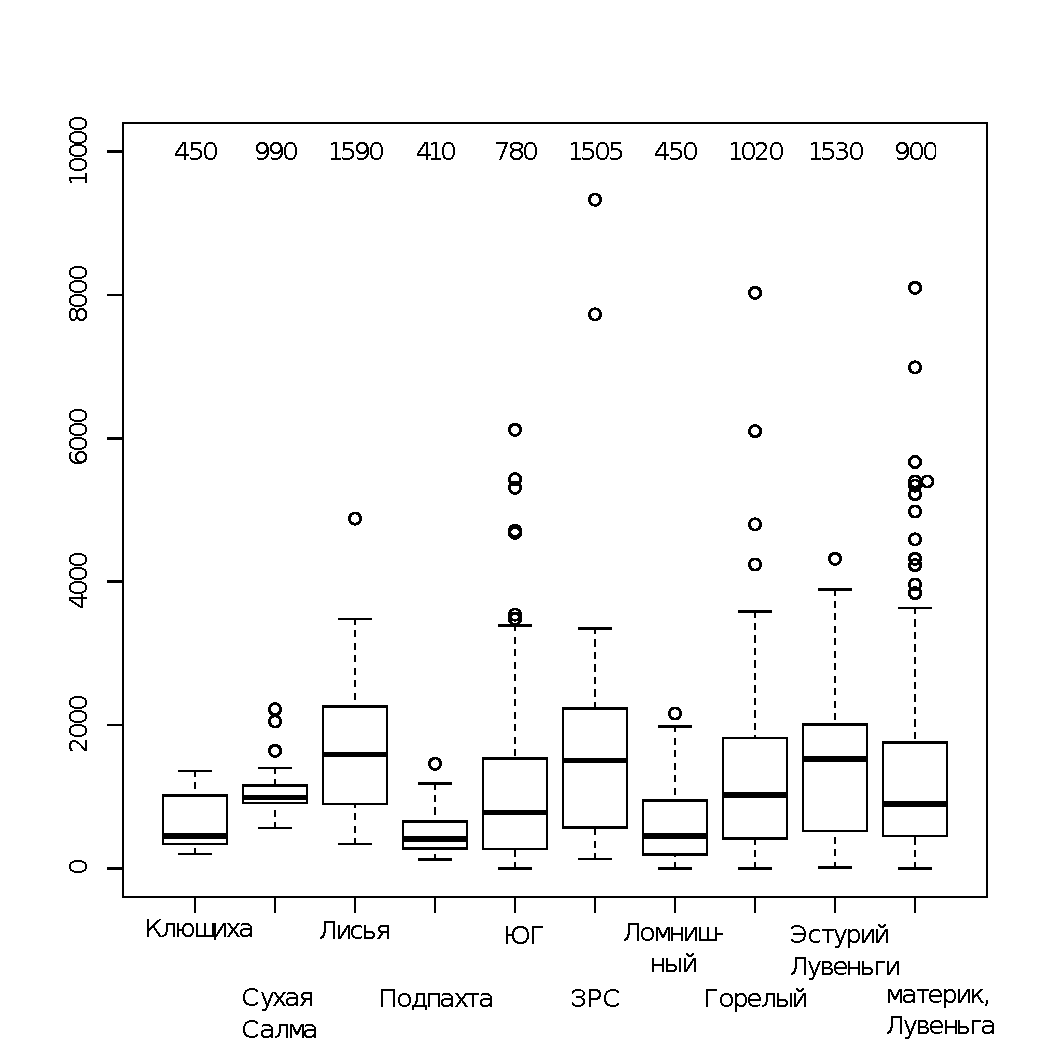
\includegraphics[width=\linewidth]{../All_N/N2_area_White1.pdf}
	\end{center}
	\end{minipage}
	\hfill
	\begin{minipage}[]{.48\linewidth}
	{\small Б}
	\begin{center}
		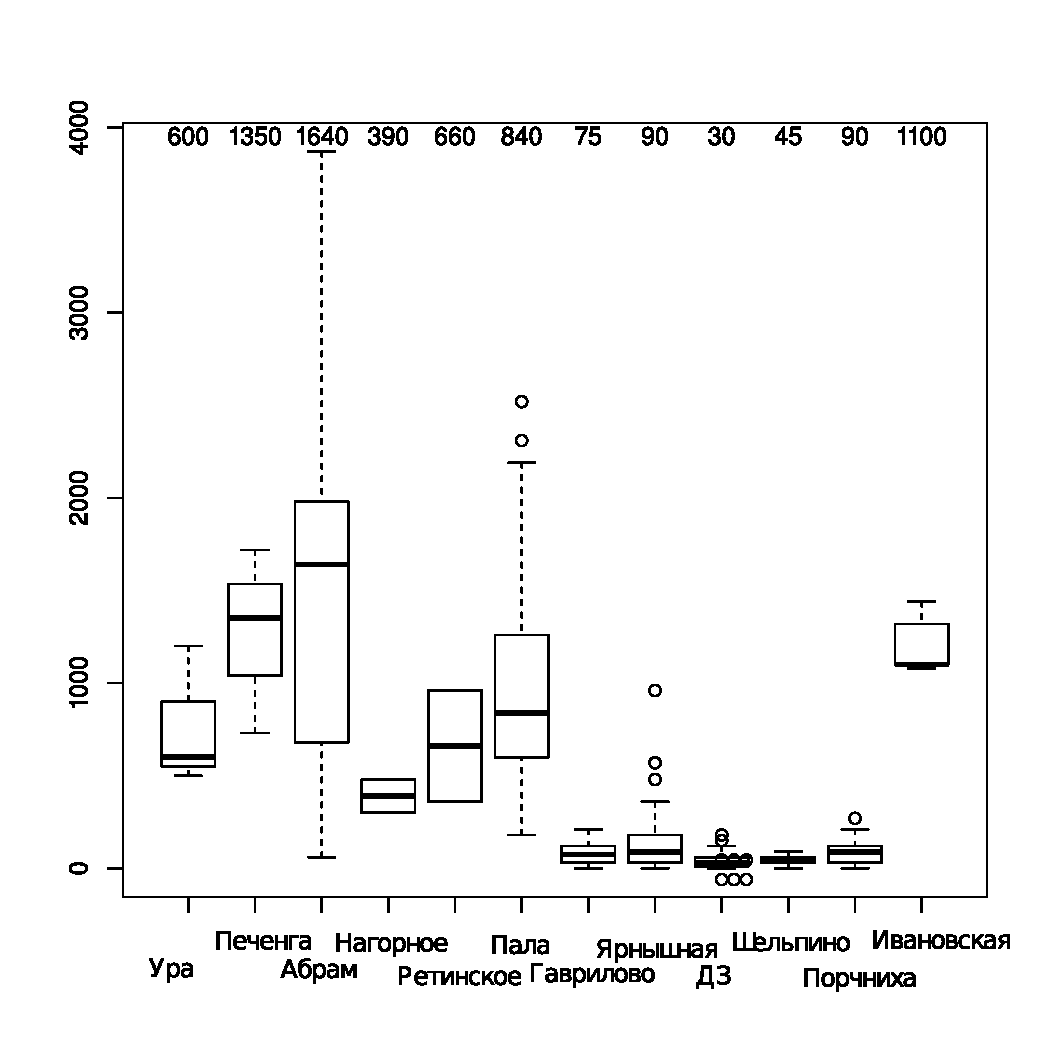
\includegraphics[width=\linewidth]{../All_N/N2_area_Barents1.pdf}
	\end{center}
	\end{minipage}
	\hfill
	\caption{Варьирование средней численности {\it Macoma balthica} в поселениях Кандалакшского залива Белого моря (А) и Мурманского побережья Баренцева моря (Б)}
	{\footnotesize Примечание: По оси абсцисс --- численность {\it M.~balthica}, ~экз./м$^2$.\\
	На графике: жирная горизонтальная линия --- медиана, границы <<ящика>> --- 1 и 3 квартили, <<усы>> --- $1,5$ интерквартильного расстояния, точки - значения выпадающие за $1,5$ интерквартильных расстояния.
Числа в верхней части графика --- медианное значение численности {\it M.~balthica}, экз./м$^2$.\\
 ЮГ~--- Южная губа о.~Ряшков, ЗРС~--- Западная Ряшкова Салма, ДЗ~--- Дальне-Зеленецкая губа}
	\label{ris:N_area}
	\end{figure}

Наиболее часто встречаются поселения со средней численностью $700-800$~экз./м$^2$.
Отдельные районы Кандалакшского залива Белого моря не отличались по средней численности маком ($Kruskal-Wallis\ \chi^2 = 5,6$, $p = 0,2$).
Размах варьирования средней биомассы был от $1,1$~($25$\%)~г/м$^2$ (б.~Клющиха, $2006$~год) до $177,9$~($9$\%)~г/м$^2$ (о.~Горелый, $2004$~год)

Минимальная средняя численность составляла $30$~экз./м$^2$ (г.~Дальнезеленецкая), что сравнимо с показателями для Белого моря. 
Максимальная средняя численность была значительно меньше, чем Беломорская --- $3350$~экз./м$^2$ (Абрам-мыс) (рис~\ref{ris:N_area}, Б).
Среди исследованных наиболее часто встречались поселения со средним обилием менее $100$~экз./м$^2$.
Для Мурманского побережья Баренцева моря показаны различия между отдельными районами: Западным, Восточным Мурманом и Кольским заливом (\cite{Guryanova_Ushakov_1929, Guryanova_et_al_1930}). 
Это подтверждается нашими данными по размаху варьирования среднего обилия в пределах районов ($Kruskal-Wallis\ \chi^2 = 17,6$, $p = 0,00015$).
Средняя биомасса маком в Баренцевом море варьировала от $13,0~(53\%)$~г/м$^2$ (Гаврилово) до $216,5~(25\%)$~г/м$^2$ (Абрам-мыс). Средняя биомасса в Кольском заливе была выше, чем на Восточном Мурмане ($Kruskal-Wallis~\chi^2 = 6,8$; $p = 0,009$).

\subsection*{Глава 6. Размерная структура поселений \textit{Macoma~balthica}}
В Белом море наиболее распространенный вариант динамики размерной структуры в поселениях {\it M.~balthica} это чередование бимодальной и мономодальной размерных структур.
Мономодальная структура обычно формируется на фоне практически полной элиминации крупных особей при пополнении поселения новой генерацией маком.
В дальнейшем, если новое пополнение происходит быстрее, чем предыдущая генерация элиминирует, то формируется бимодальная размерная структура.
Среди 6 мониторинговых участков в Кандалакшском заливе Белого моря для двух из них --- в Южной губе острова Ряшков и на о. Ломнишный --- динамика размерной структуры принципиально отличалась, и мы ежегодно видим мономодальное распределение особей по размерам с доминированием мелких особей.

В Баренцевом море на исследованных участках были представлены все возможные варианты размерной структуры: мономодальное (участки: Арабм-мыс СГЛ, Пала-губа СГЛ, губа Гаврилово СГЛ), бимодальное (участки: Абрам-мыс НГЛ, Пала-губа НГЛ, губа Ярнышная, губа Дальне-Зеленецкая СГЛ, губа Порчниха СГЛ) и практически равномерное (участки: губа Гаврилово НГЛ, губа Дальне-Зеленецкая ВГЛ и НГЛ, губа Шельпино ВГЛ и СГЛ, губа Ивановская ВСЛ) распределение особей по размерам. 
Мономодальное распределение особей по размерам наблюдается либо при доминировании мелких особей длиной $3-5$~мм, либо при доминировании крупных --- $12-18$~мм.
При бимодальном распределении обычно первую моду формировали мелкие макомы длиной $2-5$~мм, а вторую --- моллюски длиной более $10$~мм.

\subsection*{Глава 7. Линейный рост \textit{Macoma~balthica}}

На литорали Баренцева моря особи \textit{M.~balthica} гетерогенны по скорости роста. По   итогам   классификации   было   выделено   три   группы   маком,   отличающиеся   по характеру роста (рис.~\ref{ris:Barents_clusters_gorizonts_all}).
    \begin{figure}[]
        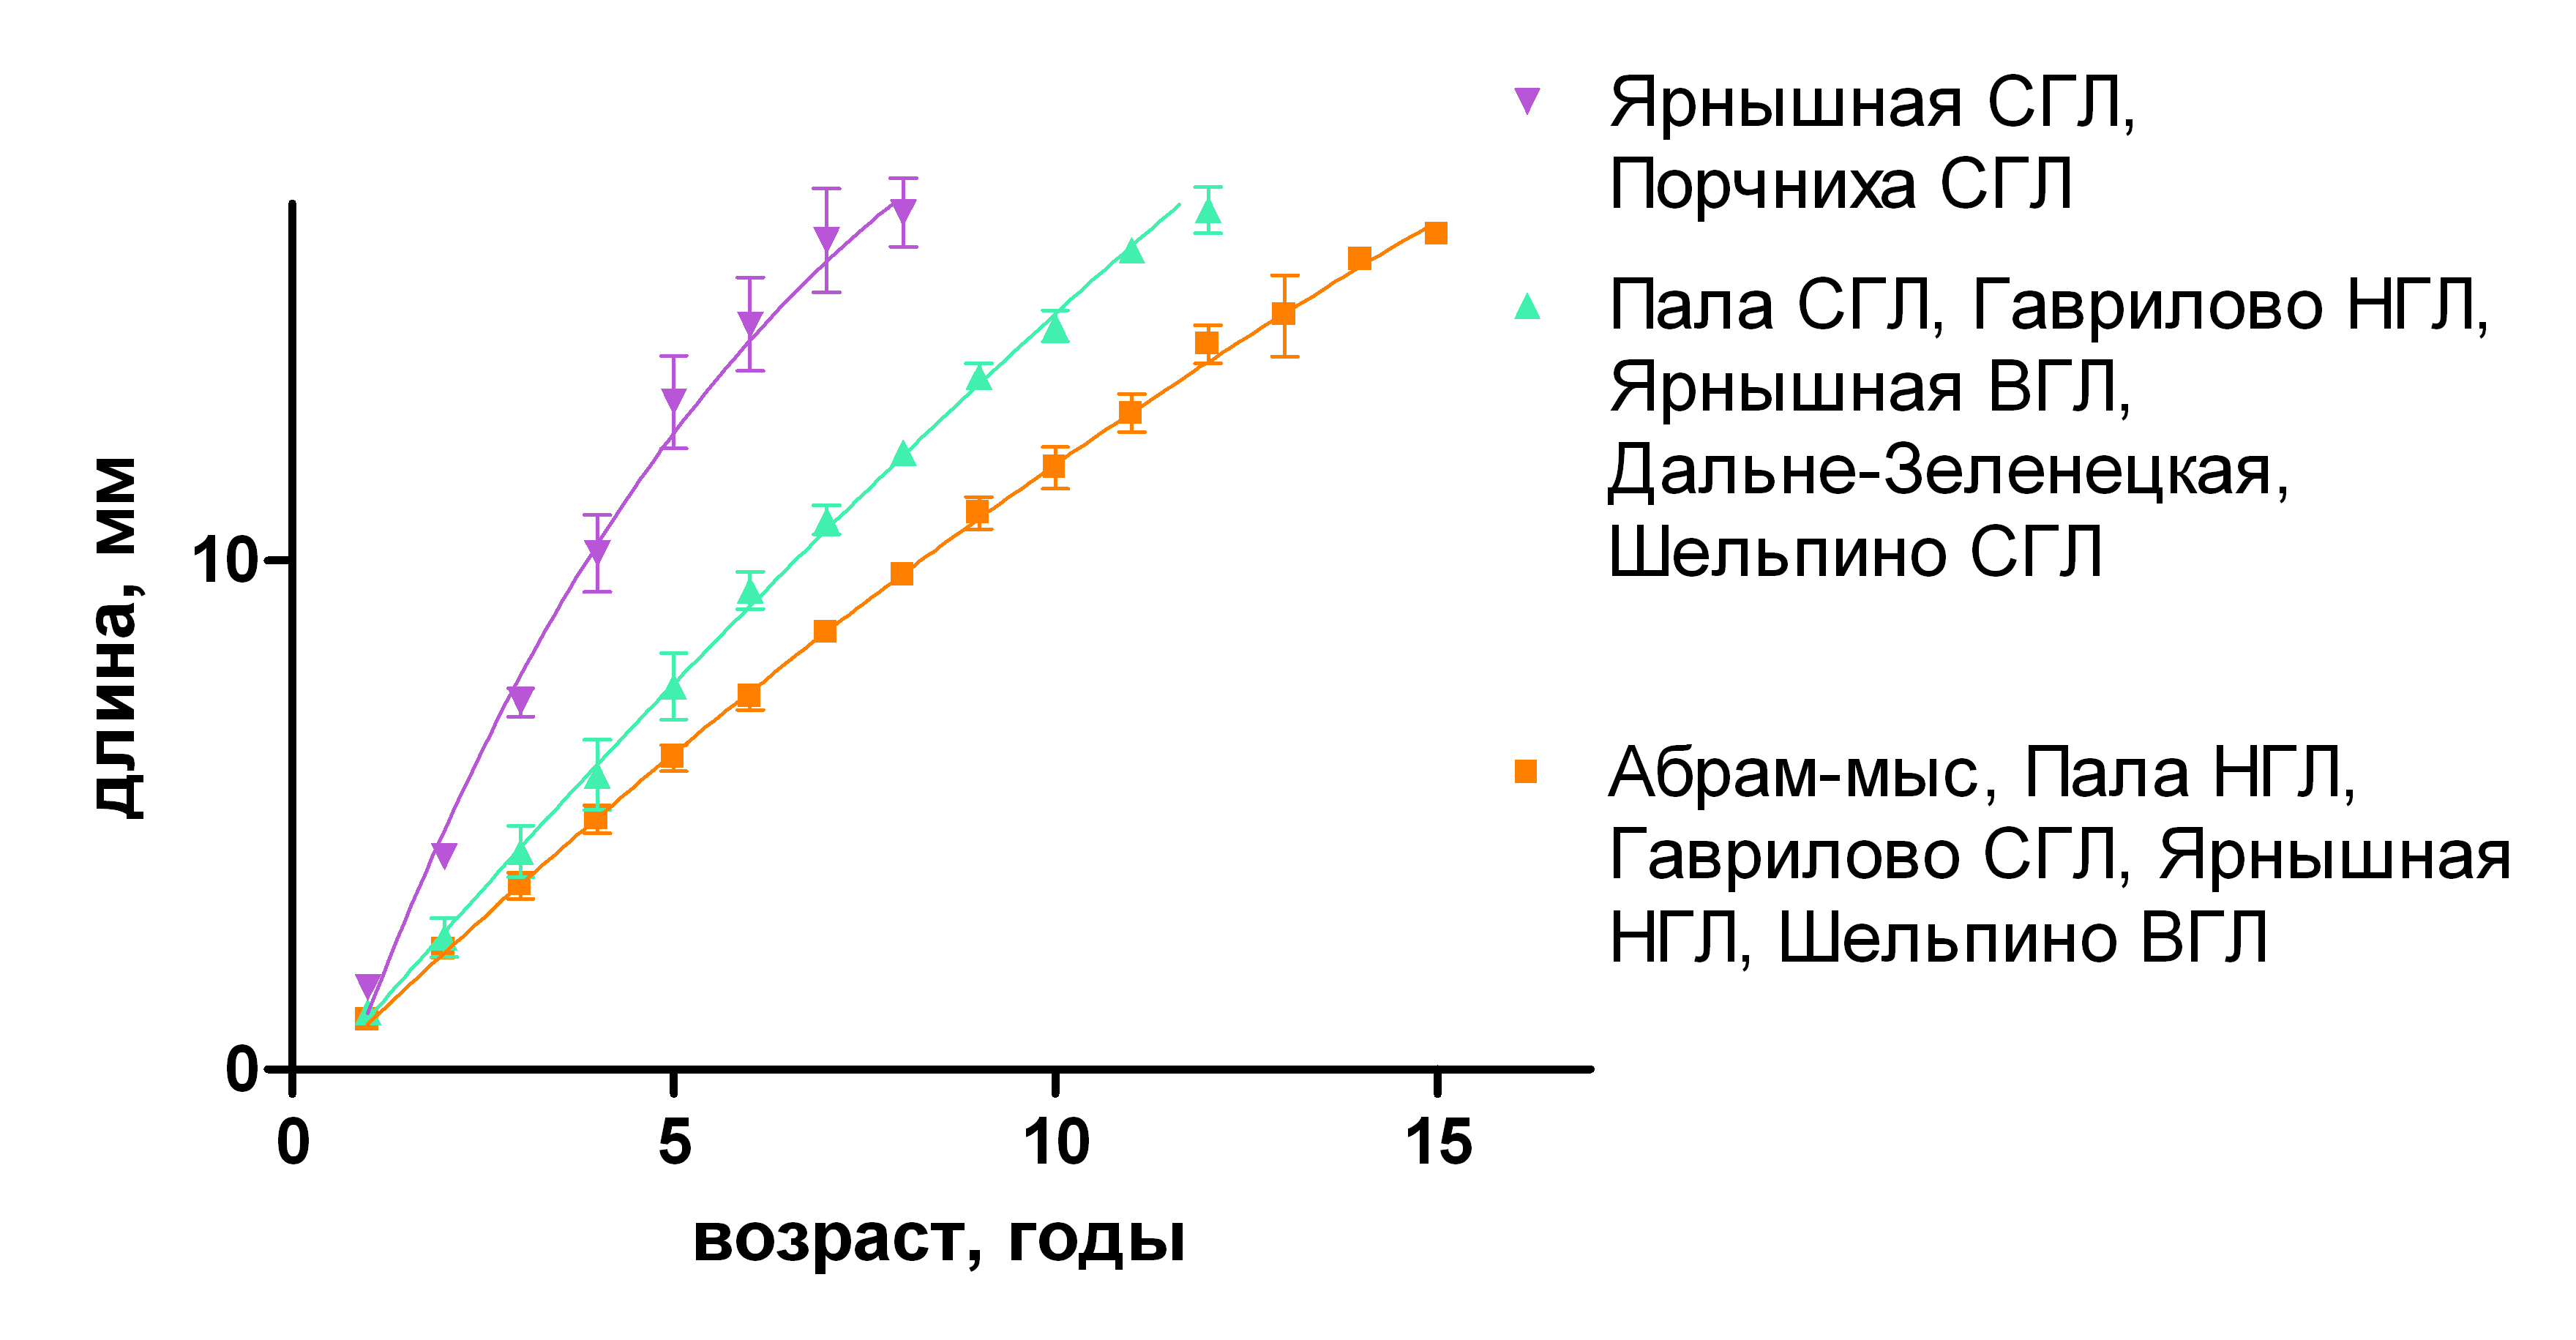
\includegraphics[width=\textwidth]{../Barenc_Sea/growth_from_MSc/rost_clusters_all.jpg}
    \caption{Модели роста, передающие  принципиальные свойства вариации характера линейного роста маком в изученных местообитаниях}
    \label{ris:Barents_clusters_gorizonts_all}
    \end{figure}
Первая группа — особи с наименьшей скоростью роста достигали длины $16,4$ мм за $14$ лет, обитавшие на относительно более низком уровне осушки. 
Макомы с промежуточной   скоростью   роста   вырастали   за   $13$   лет   $до   19,3$   мм.   
Особи   с   максимальной скоростью роста за $9$ лет достигали длины $18$ мм.

При сравнении кривых роста не было отмечено сходства роста у особей из одного поселения или с одного уровня осушки. 
Однако анализ среднего годового прироста в различных размерных группах показал, что в более восточных поселениях данный показатель выше, чем в более западных (рис.~\ref{ris:prirost_otklik}). 
	\begin{figure}[]
		\begin{minipage}[b]{.5\linewidth}
		%Фигурка в первом ряду слева размер отведенный под весь этот объект -- 0.46 от ширины строки
		%Параметр [b] означает, что выравнивание этих министраниц будет по нижнему краю
				{\small А}
			\begin{center}
				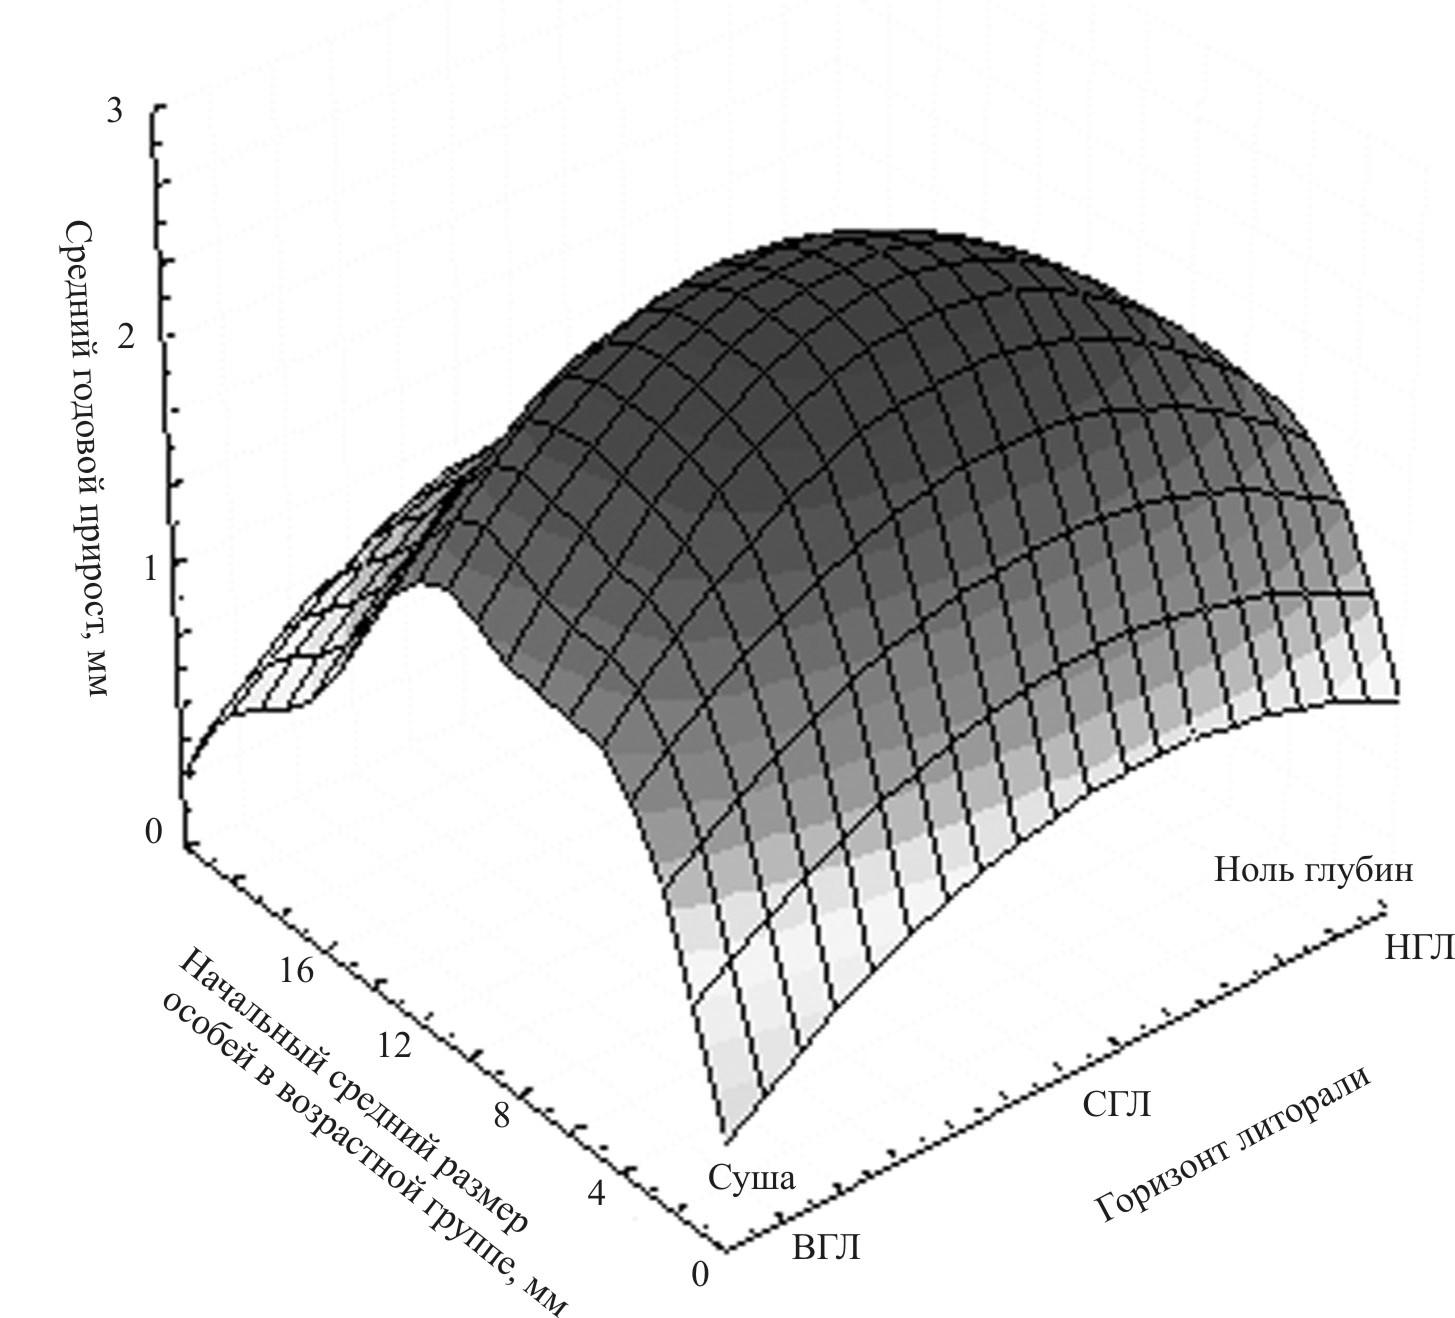
\includegraphics[width=\textwidth]{../Barenc_Sea/growth_from_MSc/prirost_otklik_mareography.jpg}
			\end{center}
		\end{minipage}
	\hfil %Это пружинка отодвигающая рисунки друг от друга
		\begin{minipage}[b]{.5\linewidth}
				{\small Б}
			\begin{center}
				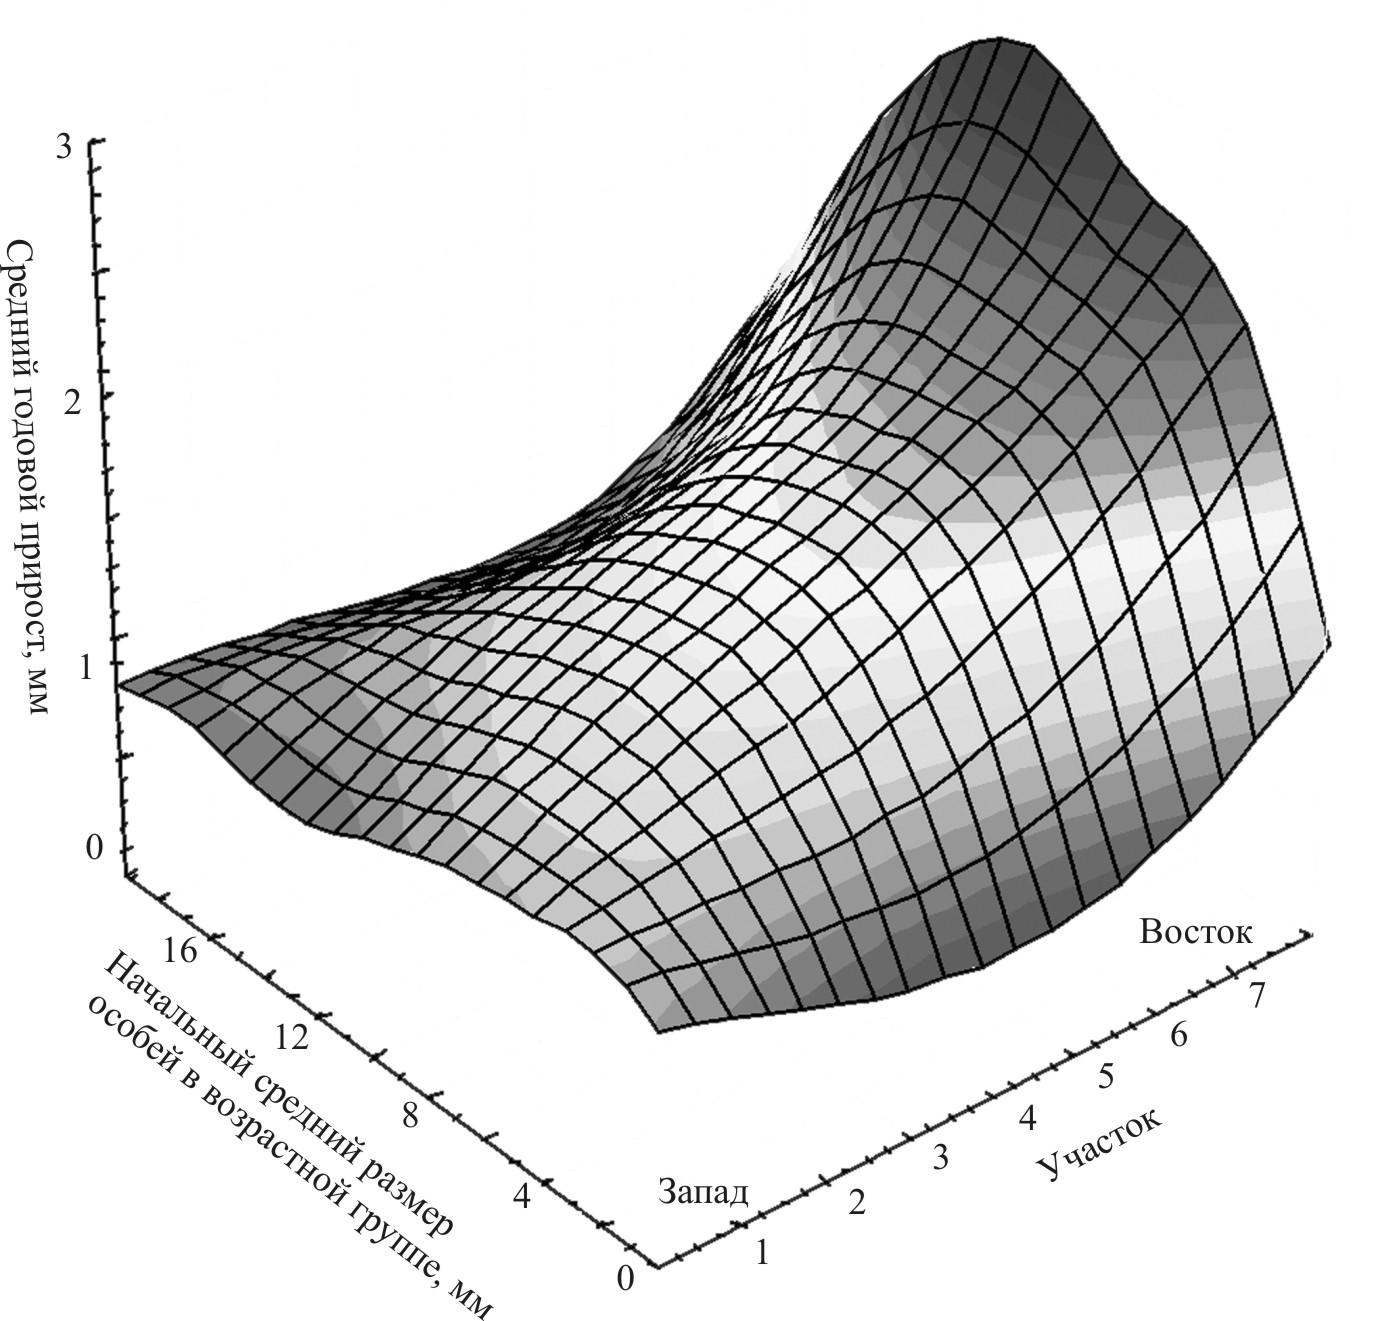
\includegraphics[width=\textwidth]{../Barenc_Sea/growth_from_MSc/prirost_otklik_geography.jpg}
			\end{center}
		\end{minipage}
	\caption{Характер изменений средней величины годового прироста особей {\it Macoma balthica} возрастной группы в зависимости от начальной средней длины их раковин, мареографического уровня обитания (A) и условного смещения участка по побережью Мурмана на восток (Б)}
\footnotesize{Примечания: Участки: 1 --- Абрам-мыс, 2 --- Пала-губа, 3 --- Гаврилово, 4 --- Ярнышная, 5 --- Дальнезеленецкая, 6 --- Шельпино, 7 --- Порчниха\\
ВГЛ --- верхний горизонт литорали, СГЛ --- средний горизонт литорали, НГЛ --- нижний горизонт литорали}
	\label{ris:prirost_otklik}
	\end{figure}
Также было показано, что в среднем горизонте литорали средний годовой прирост оказывается выше, чем в верхнем и нижнем.
Данные закономерности были выражены в разной степени у особей, отличающихся по длине раковины.
Во всех случаях наибольший средний годовой прирост наблюдали у особей с длиной раковины $6 - 9$~мм.



\subsection*{Глава 8. Динамика обилия \textit{Macoma~balthica}}

На основании долговременных рядов (время наблюдения от 7 до 20 лет) была описана динамика обилия поселений \textit{M.~balthica} в вершине Кандалакшского залива Белого моря и в губе Дальне-Зеленецкой Баренцева моря.

На протяжении $20$ лет во всех исследованных Беломорских поселениях \textit{M.~balthica} были отмечены колебания численности с амплитудой, достигающей двух порядков (от сотен до десяти тысяч особей).
При менее длительных наблюдениях динамика обилия маком в поселениях могла быть относительно стабильной.
Локальные повышения численности особей \textit{M.~balthica} были отмечены в $1999-2000$, $2004-2005$ и $2008$ годах.
Однако только увеличение численности моллюсков в $1999-2000$ привело к формированию стабильных поселений маком с высокой плотностью, в остальных случаях локальное повышение численности нивелировалось за следующий год.

Единственное поселение в Баренцевом море, где были проведены многолетние наблюдения~--- в губе Дальне-Зеленецкой, характеризовалось низкой численностью особей (десятки особей) и относительной стабильностью динамики численности. 

\subsection*{Глава 9. Количественные характеристики формирования спата в поселениях \textit{Macoma~balthica} на литорали губы Чупа (Белое море)} 

Оседание спата широко варьирует в пределах локальных акваторий.
На исследованных участках численность спата варьировала от $4$ до $10$~тыс.~экз./м$^2$.
По результатам дисперсионного анализа как численность взрослых особей ($F = 8,0; p = 0,01$), так и уникальный набор условий каждого участка ($F = 9,93; p = 0,002$) достоверно влияют на количество маком, осевших в поселении, причем вариабельность от участка к участку выше, чем вариабельность, обусловленная высокой или низкой численностью взрослых особей в поселении. 

\subsection*{Глава 10. Динамика пополнения поселений \textit{Macoma~balthica} в Белом море}

Численность годовалых особей значительно варьирует год от года: от $0$ дл $5500$~экз./м$^2$.
При этом именно флуктуации численности годовалых особей во-многом определяют изменения общего обилия маком ($Spearman\ \rho = 0,83, p < 0,0001$).

Если при размножении формируется общий личиночный пул, а в дальнейшем на выживаемость влияют зимние условия, можно предположить, что географически близкие поселения должны пополнятся синхронно.
По результатам корреляционного анализа Мантеля в поселении на о.~Горелом успешные пополнения происходили синхронно с поселениями на материковой литорали в Лувеньге ($Mantel r = 0,96, p = 0,009$) и двумя участками литорали на о.~Ряшкове (Южная губа ($Mantel r = 0,52, p = 0,004$) и Западная Ряшкова салма ($Mantel r = 0,99, p = 0,001$)).
Также был синхронным характер динамики поселений в Южной губе о.~Ряшкова с участком в эстуарии р.~Лувеньги ($Mantel r = 0,79, p = 0,001$), и участка в Западной Ряшковой Салме с Лувеньгой ($Mantel r = 0,97, p = 0,002$).

\subsection*{Глава 11. Обсуждение результатов}
Исследованные нами участки биотопически разнородны и относительно полно характеризуют разнообразие илисто-песчаных литоралей в исследованных акваториях, а отмеченные нами виды являются характерным окружением для \textit{M.~balthica} (\cite{Derugin_1915, Guryanova_et_al_1928, Guryanova_Ushakov_1929, Guryanova_et_al_1930,Babkov_Golikov_1984, Naumov_Fedyakov_1993, Chertoprud_et_al_2004, Naumov_2006, Gerasimova_et_al_2010, Derevenschikov_Kravets_2010, Stolyarov_2010}, то есть мы имели дело с типичными для данного региона биосистемами.

\subsubsection*{Структура поселений \textit{Macoma~balthica}}
\paragraph{Численность}
Полученные для Белого и Баренцева данные об обилии \textit{M.~balthica} хорошо согласуются с литературными данными об этих регионах.
Для сравнения наших данных по Белому и Баренцеву морям с данными по обилию маком в других частях европейской части ареала была собрана опубликованная информация о среднем обилии особей {\it M.~balthica} в различных акваториях (рис.~\ref{ris:NB_areal},~А).
	\begin{figure}[]
		\begin{minipage}[b]{.5\linewidth}
		%Фигурка в первом ряду слева размер отведенный под весь этот объект -- 0.46 от ширины строки
		%Параметр [b] означает, что выравнивание этих министраниц будет по нижнему краю
	{\small А}
			\begin{center}
			    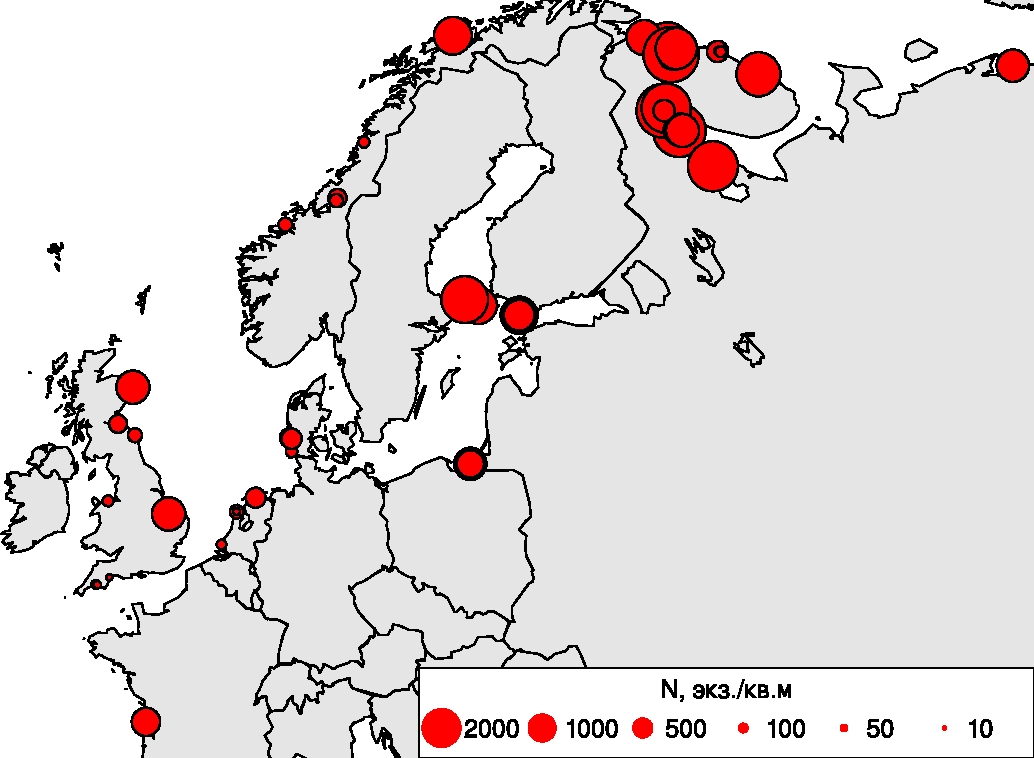
\includegraphics[width=\textwidth]{../macrodistribution/Nmean_ru1.pdf}
			\end{center}
		\end{minipage}
	\hfil %Это пружинка отодвигающая рисунки друг от друга
		\begin{minipage}[b]{.5\linewidth}
			{\small B}
			\begin{center}
				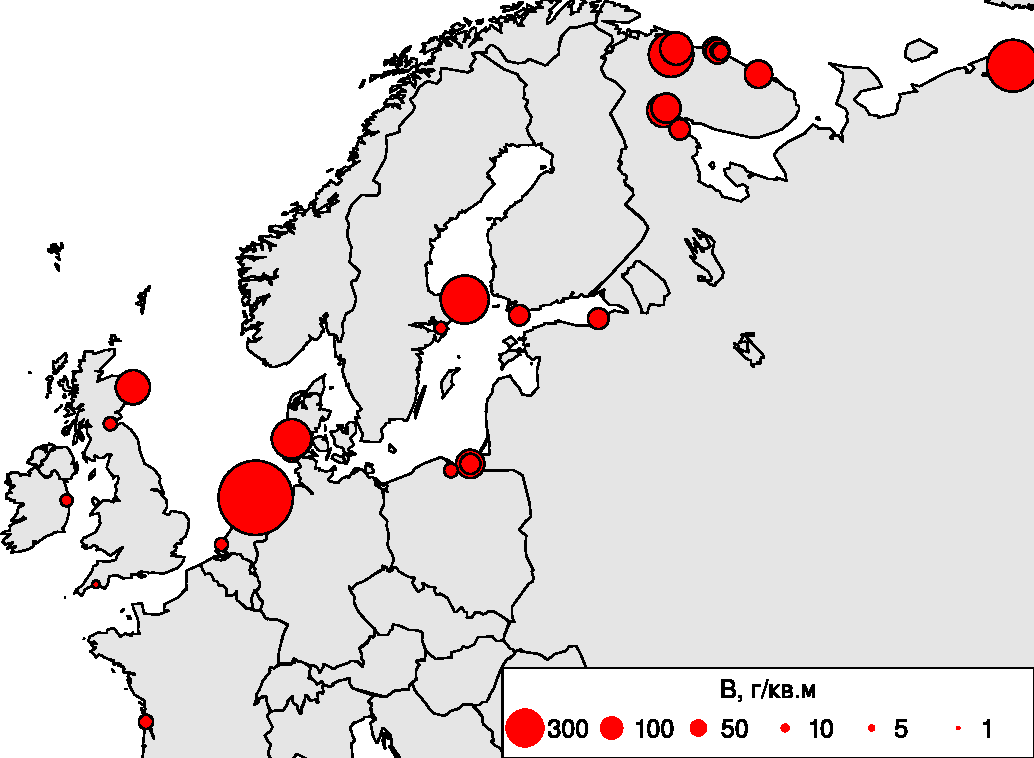
\includegraphics[width=\textwidth]{../macrodistribution/Bmean_ru1.pdf}
			\end{center}
		\end{minipage}
	\caption{Средние численность (А) и биомасса(Б) {\it Macoma balthica} в европейской части ареала}
	\label{ris:NB_areal}
	\end{figure}
Численность {\it M.~balthica} на Западном Мурмане и в Кольском заливе была сравнима с численностями моллюсков в Белом море, Балтийском море и северной части Норвежского моря (\cite{Semenova_1974, Aschan_1988, Maximovich_et_al_1991, Bonsdorff_et_al_1995, Bostrom_Bonsdorff_2000, Oug_2001, Laine_et_al_2003, Khaitov_et_al_2007, Varfolomeeva_Naumov_2013}).
Численности маком, сходные по величине с отмеченными на Восточном Мурмане, характерны для Норвежского и Северного морей (включая Ваттово море) (\cite{Brady_1943, Sneli_1968, Stromgren_et_al_1973, Beukema_1976, Jensen_Jensen_1985, Jensen_et_al_1985, Madsen_Jensen_1987, Beukema_1979, Zwarts_Wanink_1993, Reise_et_al_1994}) (рис.~\ref{ris:NB_areal}).

Численность в сублиторали Восточного Мурмана (Ивановская губа) была выше, чем численность моллюсков на литорали.
В верхней сублиторали Печерского моря (восточная часть Баренцева моря, \cite{Denisenko_et_al_2003}) численность маком была в два раза ниже, чем отмеченная нами, однако также была значительно выше обилия данного вида на литорали Восточного Мурмана.
Более высокие численности маком в верхней сублиторали относительно литорали отмечены для некоторых участков в Белом море (\cite{Semenova_1974}), хотя чаще отмечается обратный эффект (\cite{Semenova_1974, Maximovich_et_al_1991}).

Максимальная средняя численность маком монотонно увеличивается с широтой.
Таким образом, распределение вида {\it M.~balthica} в европейской части ареала может быть описано как увеличивающееся к северу (<<ramped north>>) (\cite{Sagarin_Gaines_2002}).

\paragraph{Биомасса}
Максимальная биомасса была отмечена в центральной части ареала~--- в Северном и Балтийском морях (рис.~\ref{ris:NB_areal}).
На южном краю ареала биомасса ожидаемо снижается, в то время как в северной части ареала биомасса сравнима со средними значениями в центральной части ареала, хотя и не достигает максимальных.
Таким образом, распределение поселений с различной биомассой в целом соответствует гипотезе об обилии в центре (\cite{Sagarin_Gaines_2002}).

%	\subsubsection*{Особенности структуры поселений {\it Macoma balthica}}
\paragraph{Размерная структура}
В исследованных нами поселениях размерная структура \textit{M.~balthica} значительно варьирует, однако при достаточно высокой численности моллюсков мы наблюдаем две наиболее характерные ситуации: мономодальное распределение особей по размерам чаще всего с преобладанием молодых особей, и бимодальное распределение.

Рассматривая динамику размерной структуры, можно говорить о  двух ситуациях, которые мы наблюдали в исследованных поселениях.
Наиболее распространена ситуация, в которой наблюдается смена типа структуры со временем. 
Сначала в поселении наблюдается мономодальная структура с преобладанием относительно молодых, и со временем мы можем наблюдать смещение модального класса по оси размеров. 
Через несколько лет происходит следующее успешное пополнение поселения молодью и формируется бимодальное распределение.
Со временем происходит элиминация старших особей и, в зависимости от периода через который происходит следующее успешное пополнение поселения молодью, мы либо продолжаем наблюдать бимодальное распределение, либо оно вновь становится мономодальным.
Такой тип динамики отмечен нами для всех поселений в районе Лувеньгских шхер, Западной Ряшковой салмы  и для Дальнего пляжа губы Дальнезеленецкая.
Подобная картина была ранее описана для Сухой салмы в губе Чупа Белого моря (\cite{Maximovich_et_al_1991}).
В Балтийском море описан аналогичный тип динамики (\cite{Segerstrale_1969}).

Другой вариант динамики размерной структуры, по-видимому, менее распространен.
Он выглядит как ежегодное повторение мономодальной размерной структуры в течение нескольких лет.
Такой вариант был описан для поселений \textit{M.~balthica} в Южной губе о.~Ряшкова и на о.~Ломнишном.
Интересно отметить, что оба поселения находились под влиянием хищной улитки \textit{Amauropsis islandica} (\cite{Aristov_Granovich_2011}).
Однако для того чтобы аргументированно говорить о влиянии хищников, необходимы отдельные исследования.
Сходный тип динамики был описан для бухты Клющиха в губе Чупа Белого моря (\cite{Maximovich_et_al_1991, Gerasimova_Maximovich_2013}.
Все участки, на которых описан подобный тип развития поселения, сходны по топическим условиям~--- песчаный пляж с минимальным заилением.
Это подтверждает предположение, высказанное ранее (\cite{Gerasimova_Maximovich_2013}), что возможность формирования такого типа динамики может быть связана с расхождением по типу питания у молодых и взрослых маком (\cite{Gerasimova_1988, Olafsson_1989}.


\subsection*{Скорость роста {\it Macoma balthica} как отражение условий обитания}
Анализ широтных изменений параметра $\omega$ подтвердил гипотезу о снижении скорости роста в северных частях ареала маком (корреляция Спирмена: $r_{s} = -0,60$, $p < 0,0001$).
Однако, в Балтийском море присутствуют поселения со скоростью роста, сравнимыми с характеристиками для арктических морей~--- Белого и Баренцева. 
По-видимому, это связано с влиянием низкой солености на скорость роста (\cite{Segerstrale_1960, Kube_et_al_1996}).

Для учета варьирования реальных ростовых характеристик мы сравнили имеющиеся в литературе данные и полученные нами данные с учетом разброса эмпирических данных относительно регрессионной модели.
Всего было использовано $33$ описания с $23$ географических точек на Европейском побережье Северной Атлантики.
Мы использовали данные о первых $6$ годах роста особей, для унификации длины сравниваемых рядов.
Было выделено $6$ групп моллюсков, различающихся по ростовым характеристикам (рис.~\ref{ris:growth_cluster_literature}).
	\begin{figure}[ht]
	\begin{center}	
		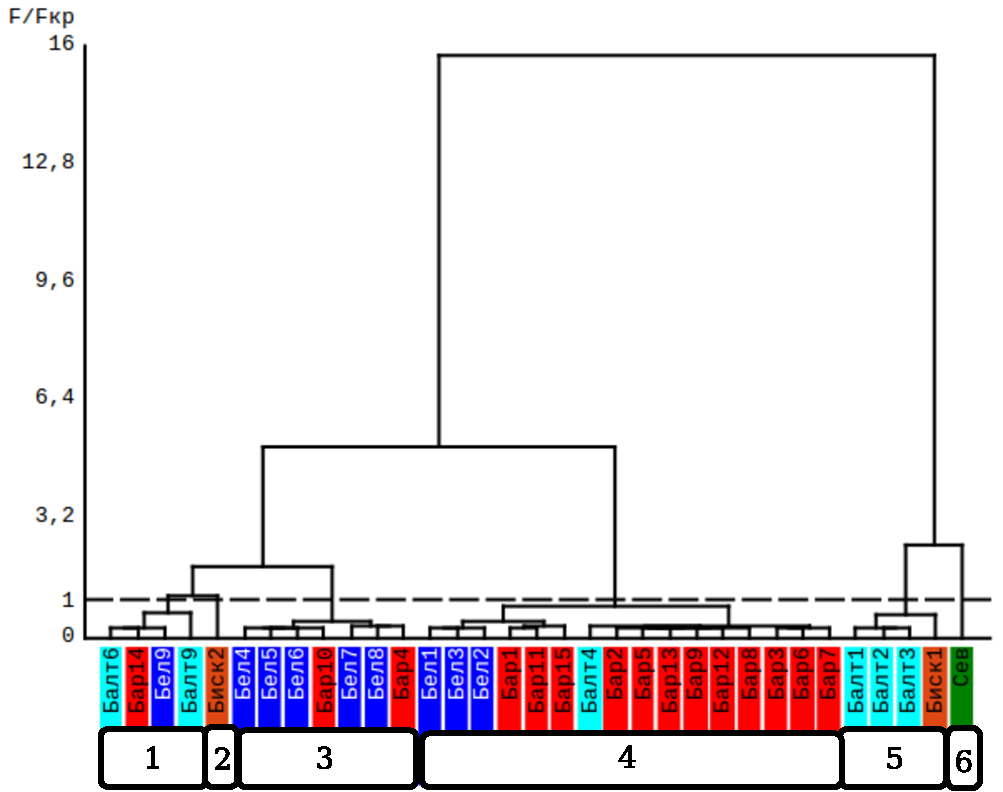
\includegraphics[height=0.4\textheight]{../Growth_sravnenie/Europe_clusters_usrednenie.pdf}
	\end{center}
		\caption{Классификация поселений маком на Европейском побережье в Северной Атлантике по моделям линейного роста}
	\footnotesize{Примечание: Дендрограмма сходства 33 рядов, аппроксимированных уравнением Берталанффи. 
Способ объединения рядов в кластеры~--- усреднение значений переменной $Y$, соответствующих одному значению $X$.
Мера сходства~--- $F/F_{kp}$ (уровень значимости $\alpha = 0,05$)\\
Моря: Балт~--- Балтийское, Бар~--- Баренцево, Бел~--- Белое, Биск~--- Бискайский залив, Сев~--- Северное.}
%Цвета: Красный~--- Баренцево море, синий~--- Белое море, голубой~--- Балтийское море, зеленый~--- Северное море, оранжевый~--- Бискайский залив}
		\label{ris:growth_cluster_literature}
	\end{figure}
Максимальная скорость роста была отмечена для группы $6$ (рис.~\ref{ris:growth_model_europe})~--- поселение в Северном море (\cite{Vogel_1959}). 
Группа $4$, в которую вошло большинство изученных нами поселений в Баренцевом море, характеризуется минимальной скоростью роста.
Также в эту группу вошла часть Беломорских поселений (\cite{Semenova_1970}) и одно поселение в Балтийском море (\cite{Bergh_1974}).
Часть исследованных поселений в Баренцевом море отличалась более высокой скоростью роста, и попала в группы $3$ (<<Беломорский>> кластер) и $1$ (Беломорские, Балтийские и Бренцевоморские поселения).
Интересно отметить, что более южные поселения (входщие в состав групп $2$ и $5$~--- <<Балтийский>> кластер), в Бискайском заливе (\cite{Bachelet_1980}), характеризуются более низкой скоростью роста , чем в центральной части ареала (рис.~\ref{ris:growth_model_europe}).
Данный результат хорошо согласуется с <<гипотезой об обилии в центре>> (<<abindant-centre hypothesis>>, \cite{Sagarin_et_al_2006}) и ранее проведенными исследованиями (\cite{Beukema_Meehan_1985, Hummel_et_al_1998}).

\subsection*{Долговременные тренды в поселениях \textit{Macoma~balthica}}
Изучение плотностнозависимых процессов методом частных корреляций показало, что подобные процессы второго порядка характерны только для поселений в Южной губе о.~Ряшкова и на материковой литорали в Лувеньге (достоверные значений $PRCF[2]$, причем в Южной губе $PRCF[2] > PRCF[1]$)
Предположительно, это может быть воздействие хищников.

Для оценки пространственных масштабов синхронности поселений было сравнение проведено сравнение характера динамики численности маком в поселениях в вершине Кандалакшского залива (авторские данные) и в губе Чупа (\cite{Maximovich_et_al_1991, Gerasimova_Maximovich_2013, Varfolomeeva_Naumov_2013}) методом корреляционного анализа Мантеля.
Синхронность динамики обилия демонстрировали большинство поселений (рис.~\ref{ris:mantel}).
	\begin{figure}[]
	\begin{center}	
		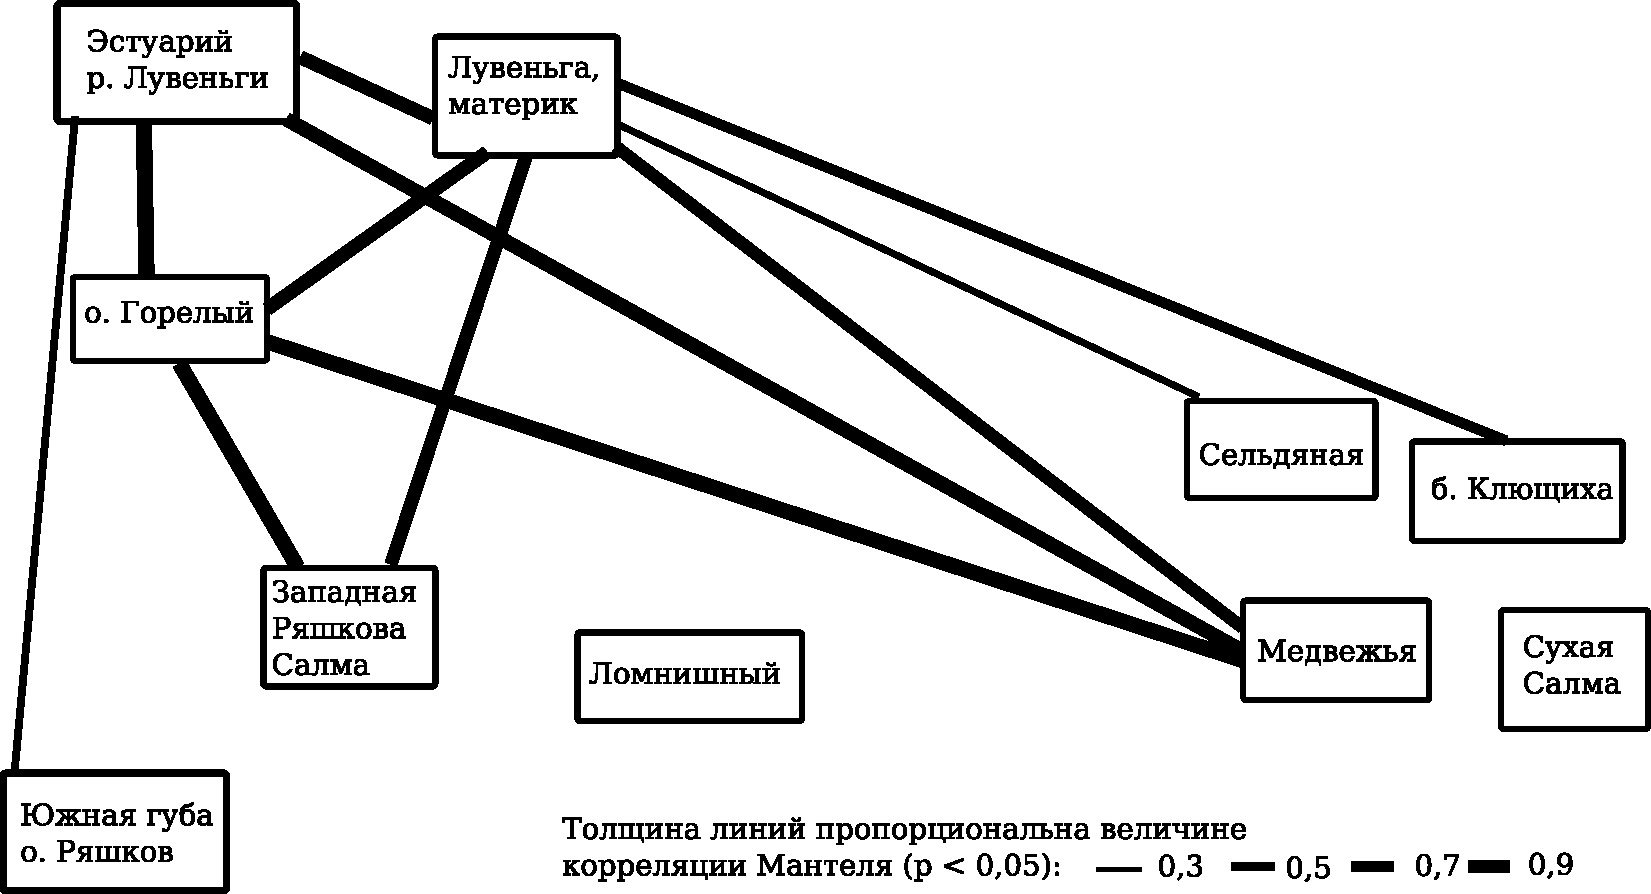
\includegraphics[width=\textwidth]{../White_Sea/dynamic_N_N1/mantel1.pdf}
	\end{center}
		\caption{Синхронность поселения \textit{Macoma balthica} в Белом море}
		\label{ris:mantel}
	\end{figure}
Расстояние между поселениями варьировало от $1$ до $100$~км.
Таким образом, можно предположить, что динамика обилия маком подвержена влиянию глобальных абиотических факторов, первым из которых может быть температура. 
Для проверки влияния температуры на динамику обилия \textit{M.~balthica} было проведено моделирование с использованием линейных моделей. 
Полная модель включала в себя независимую переменную логарифм средней численности маком в данный год ($\log(N_{t1})$) и независимые факторы: логарифм численности маком в предыдущий год ($\log(N_{t})$), среднелетнюю температуру в предыдущий год ($T_{st}$) как отражение условий созревание гонад и формирования спата и среднезимнюю температуру в текущий год ($T_{wt1}$) как отражение критических условий первой зимы для сеголетков. 
В дальнейшем модель была редуцирована (полная и минимальная модели, ANOVA: $F = 0,43$; $p = 0,79$) и в минимальную модель в качестве факторов входили $\log(N_{t})$ и $T_{wt1}$: $\ln(N_{t1}) = 1,96 + 0,60 \times \ln(N_{t}) - 0,09 \times T_{wt1}$ ($F = 37,04$; $p < 0,0001$. $R^2 = 0,6$)
Построенная модель удовлетворяла условиям применимости линейных моделей: отсутствия автокорреляций (критерий Дарбина-Уотсона: $1,71$; $p = 0,27$), нормальности распределения остатков (критерий Шапиро-Уилка: $W = 0,99$; $p = 0,86$) и гомогенности дисперсий (критерий Бройша-Пагана: $BP = 5,25$; $p-value = 0,15$). 

Полученные данные о влиянии зимней температуры противоречат нашей исходной гипотезе о том, что холодные зимы в Белом море критичны для маком. 
Результаты моделирования позволяют говорить о том, что обилие маком увеличивается после более холодных зим и уменьшается после относительно теплых. 
Данный результат хорошо согласуется с результатами полученными Бьёкема с соавторами (\cite{Beukema_et_al_1998, Beukema_et_al_2009}) для Ваттового моря, где основной механизм влияния температуры был через регулирование численности беспозвоночных хищников.  
Однако считается, что роль хищников снижается в более полярных сообществах (\cite{Pianka_1966, Freestone_et_al_2011}). 
По-видимому, в Белом море уменьшение обилия маком после теплых зим связано с тем, что при более теплых зимах ледостав менее стабилен, и литораль во время отлива оказывается напрямую подвержена воздействию отрицательных температур воздуха, в то время как в холодные зимы стабильный ледовый покров создает изолирующий слой, и колебания температуры подо льдом оказываются значительно ниже (\cite{Kuznecov_1960}).
%\subsection*{Заключение}
%	\chapter*{Заключение}		
\addcontentsline{toc}{chapter}{Заключение}	% Добавляем его в оглавление

Двустворчатый моллюск \textit{Macoma balthica} является типичным представителем литоральной фауны в Белом и Баренцевом морях. 
В Белом море данный вид формирует плотные скопления, причем поселения в Кандалакшском заливе характеризуются максимальной средней численностью в европейской части ареала вида.
В Баренцевом море \textit{M.~balthica} на литорали Западного Мурмана и Кольского залива также формирует плотные поселения, в то время как на литорали Восточного Мурмана численность данного вида редко превышает $100$~экз./м$^2$.

Динамика размерной структуры поселений {\it M.~balthica} в Белом и Баренцевом представлена двумя типами.
Более распространенный вариант: чередование бимодального и мономодального распределение особей по размерам. 
При этом первый пик формируют молодые особи (обычно длиной до 5~мм), а в случае бимодальной добавляется второй модальный класс из взрослых особей (в Белом море длиной 9 -- 12~мм, в Баренцевом 10 -- 17~мм). 
В Баренцевом море часто новое пополнение происходит до ухода старшей генерации и наблюдается три модальных группы. 
Такой тип динамики связан с различной успешностью ежегодного пополнения поселений молодью и, по-видимому, наличием внутривидовой конкуренции между взрослыми и молодыми особями.
В некоторых условиях формируется более редкий тип динамики с ежегодным повторением мономодальной размерной структуры. 
Возможно, это связано со специфическими условиями гидродинамики, в которых происходт разделение молодых и старых особей по способу питания и, таким образом, снижение внутривидовой конкуренции и возможность большего успеха ежегодного пополнения поселения молодью. 
Другое возможное объяснение --- формирование такого типа динамики в поселениях, находящихся под прессом хищников, которые уменьшают численность взрослых особей.

Макомы в Баренцевом море гетерогенны по скорости роста. 
Более высокая скорость роста была отмечена у особей {\it M.~balthica} обитающих в среднем горизонте литорали.
Также показано увеличение среднего годового прироста в более восточных поселениях на Мурманском побережьи.
Анализ скорости роста в европейской части ареала показывает снижение данного показателя в краевых популяциях, причем на севере это снижение более выражено.

Динамика численности поселений {\it M.~balthica} в Белом море характеризуется значительными колебаниями, связанными в первую очередь с численностью сеголетков. Изменения плотности поселений маком оказываются синхронными в пределах значительной акватории.
Численность маком оказывается выше после холодных зим, таким образом, по-видимому, основное влияние оказывают ледовые условия.
Предположительно, в более холодные зимы устойчивый ледовый покров формируется раньше и надежнее, поэтому выживаемость спата в зимний период выше, что фиксируется в наших наблюдениях, как более эффективное пополнение поселения, приводящее к увеличению общей численности {\it M.~balthica}.

Обнаружение в поселениях, обитающих в присутствии хищников, плотностно-зависимых процессов второго порядка позволяет говорить о том, что традиционно-предполагаемое минимальное влияние хищников на бентосные популяции в Арктических морях не соответствует действительности, и оказываемое на конкретное поселение воздейсвтие может быть значимо.

Численность спата на порядок варьирует в пределах незначительной акватории.
Основное влияние оказывает топология местности.
Также, по-видимому, оседание спата снижено в поселениях в высокой численностью взрослых особей {\it M.~balthica}, хотя масштабы этого явления и конкретные механизмы остаются неизвестными.




\subsection*{Выводы}
	\begin{enumerate}
%		\item Для Белого моря типичны поселения {\it Macoma balthica} с численностью  700 -- 800~экз./м$^2$ (при варьировании от 10 до 8500~экз./м$^2$). Варьирование обилия связано в первую очередь с численностью годовалых особей.
		\item Для Белого моря типичны поселения {\it Macoma balthica} с численностью в сотни экз./м$^2$ (при варьировании от единичных особей до более $8$~тыс.~экз./м$^2$). Варьирование обилия связано в первую очередь с численностью годовалых особей.
		\item Для литорали восточной части Мурманского побережья Баренцева моря типичны поселения {\it Macoma balthica} с численностью  менее 100~экз./м$^2$, и эти поселения не достигают плотностей, которые показаны для поселений на литорали Западного Мурмана и в Кольском заливе. %(при варьировании от 30 до 3350~экз./м$^2$).
		\item Среднее обилие {\it Macoma balthica} в поселениях Белого моря и Кольского залива Баренцева моря выше, чем в других частях ареала, а биомасса сравнима со значениями в центральной части ареала. 
		\item Макомы в Баренцевом море гетерогенны по скорости роста: Максимальный годовой прирост отмечен у особей среднего размера (возраста) --- $6 - 9$~мм в среднем горизонте литорали. В пределах Восточного Мурмана средний годовой прирост особей {\it Macoma balthica} увеличивается в более восточных районах по сравнению с западными.
		\item В пределах европейской части ареала особи {\it Macoma balthica} из поселений в Белом и Баренцевом морях характеризуются минимальными скоростями роста. При этом нет принципиальных различий в скорости роста беломорских и баренцевоморских маком.
		\item Численность спата {\it Macoma balthica} в Белом море может варьировать на порядок в пределах незначительной акватории (от тысяч до десятков тысяч экз./м$^2$).
		\item Динамика численности годовалых особей {\it Macoma balthica} позволяет говорить о не ежегодном успехе пополнения их поселений в Белом море.
		\item Динамика численности {\it Macoma balthica} в Кандалакшском заливе Белого моря демонстрирует элементы синхронности в поселениях, расположенных на расстоянии от 1 до 100~км. Кроме того, показано что численность маком оказывается выше в годы с холодными зимами.
		\item Динамика размерной структуры поселений {\it Macoma balthica} в Белом и Баренцевом представлена двумя типами. \\
Более распространенный вариант: чередование бимодального и мономодального распределение особей по размерам. При этом первый пик формируют молодые особи (обычно длиной до 5~мм), а в случае бимодальной добавляется второй модальный класс из взрослых особей (в Белом море длиной 9 -- 12~мм, в Баренцевом 10 -- 17~мм). В Баренцевом море часто новое пополнение происходит до ухода старшей генерации и наблюдается три модальных группы. %Такой тип динамики связан с различной успешностью ежегодного пополнения поселений молодью и наличием внутривидовой конкуренции между взрослыми и молодыми особями.
В некоторых условиях формируется более редкий тип динамики с ежегодным повторением мономодальной размерной структуры. %Возможно, это связано со специфическими условиями гидродинамики, в которых происходит разделение молодых и старых особей по способу питания и, таким образом, снижение внутривидовой конкуренции и возможность большего успеха ежегодного пополнения поселения молодью. Другое возможное объяснение --- формирование такого типа динамики в поселениях, находящихся под прессом хищников, которые уменьшают численность взрослых особей.
	\end{enumerate}



%\newpage
\begin{small}
\section*{Публикации автора по теме диссертации}
\subsubsection*{В изданиях из перечня ВАК:}
\begin{enumerate}
\item Назарова С.А. и др. Линейный рост Macoma balthica в осушной зоне Мурманского побережья Баренцева моря/\textbf{С.А. Назарова}, Е.А.  Генельт-Яновский,  Н.В. Максимович// Вестник СпбГУ, сер.3, вып.4 -- Спб. -- 2010. -- C.~35-43.
\item  Nazarova S. et al. Abundance distribution patterns of intertidal bivalves Macoma balthica and Cerastoderma edule at the Murman coast tidal flats (the Barents Sea)./ \textbf{S.~Nazarova}, E.~Genelt-Yanovsky, K.~Shunkina // Journal of the Marine Biological Association of the United Kingdom., v.~First View -- 2015. — Pp.~1-8. DOI:~10.1017/S0025315415000624
\end{enumerate}

\subsubsection*{В прочих изданиях:}
\begin{enumerate}
\item Генельт-Яновский Е.А. и др. Фаунистические комплексы, ассоциированные с поселениями инфаунных двустворчатых моллюсков на литорали Мурманского побережья Баренцева моря/ Е.А.Генельт-Яновский, \textbf{С.А.Назарова}// Материалы VI всероссийской школы по морской биологии "Биоразнообразие сообществ морских и пресноводных экосистем России" (Мурманск, 1-2 ноября 2007 года). -- Мурманск, 2007. -- С.45-46.
\item Назарова С.А. и др. Структурно-функциональные характеристики поселений \textit{Macoma balthica} L. в осушной зоне Мурманского побережья Баренцева моря/ \textbf{С.А.~Назарова}, Е.А.~Генельт-Яновский//Материалы научной конференции, посвященной 70-летию ББС им. Перцова 9-10 августа 2008 года. -- М., 2008. -- C. 81-85
\item Генельт-Яновский Е.А. и др. Сообщества илисто-песчаной литорали губы Дальне-Зеленецкая (Восточный Мурман) в 2002-2007 гг/ Е.А.~Генельт-Яновский, \textbf{С.А.~Назарова}//Материалы X научного семинара <<Чтения памяти К.М.~Дерюгина>>. --СПб. -- 2008. -- С.~16-28.
\end{enumerate}

\subsubsection*{Тезисы докладов:}
\begin{enumerate}
\item Назарова С.А. Анализ многолетней динамики структуры поселений \textit{Macoma balthica} (L., 1758) в районе Лувеньгских шхер (Кандалакшский залив Белого моря)/ \textbf{С.А. Назарова}// Аничковский вестник. Материалы XIII открытой научно-практической конференции Аничкова лицея. Математическая физика, биология, психология. -- 2003. -- \textnumero34. -- С.~55-61.
\item Назарова С.А.  и др. О флуктуациях численности \textit{Macoma balthica} L. В популяциях кутовой части Кандалакшского залива (Белое море)/ \textbf{С.А.~Назарова}, А.В.~Полоскин// Тезисы докладов VI научной сессии Морской биологической станции СПбГУ (8 февраля 2005 г.). -- СПб, 2005. -- С.51-52.
\item Генельт-Яновский Е.А. и др. Закономерности в распределении некоторых видов макробентоса литорали Мурманского побережья Баренцева моря: агрегации или градиенты?/ Е.А. Генельт-Яновский, \textbf{С.А. Назарова}, Д.С. Кобылков//Тезисы докладов IX научной сессии Морской биологической станции СПбГУ (8 февраля 2008 г.). -- СПб, 2008. -- С.~45-46.
\item Назарова С.А. и др. Структура поселений \textit{Macoma balthica} L. в осушной зоне Кольского залива и Восточного Мурмана/ \textbf{С.А.~Назарова}, Е.А.~Генельт-Яновский// X научная сессия МБС СпбГУ. Тезисы докладов. -- Спб. -- 2009. -- С.~25-27.
\item Назарова С.А. И др. Линейный рост \textit{Macoma balthica} на Мурмане: географическая или биотопическая неоднородность?/\textbf{С.А.~Назарова},  Н.В.~Максимович, Е.А.~Генельт-Яновский// XI научная сессия МБС СПбГУ. Тезисы докладов. -- Спб. -- 2010. -- С.~21. 
\item Nazarova S.A. et al. Linear growth of \textit{Macoma balthica} (North Atlantic and Arctic oceans)/ \textbf{S.A.~Nazarova}, N.V.~Maximovich// 46th European Marine biology symposium. Rovinj. Croatia. Abstracts. -- Rovinj. -- 2011. -- Pp.~46.
\item Nazarova S.A. et al. Abundance and spatial distribution of two infaunal bivalves, \textit{Macoma balthica} and \textit{Cerastoderma edule}, in the Barents sea intertidal zone./ \textbf{S.A~Nazarova}, K.V.~Shunkina, E.A.~Genelt-Yanovskiy // 49 European Marine Biology Simposium, St-Petersburg. -- 2014. -- Pp.~53
\item Poloskin A.V. No rules for \textit{Macoma}?  On the long-term temporal and spatial variation of the baltic tellins populations at the Kandalaksha bay of the White sea./ A.V.~Poloskin, \textbf{S. A. Nazarova}, D.A.~Aristov, V.M.~Khaitov, A.D.~Naumov.// 49 European Marine Biology Simposium, St-Petersburg. -- Pp.~54
\item Nazarova S.A. \textit{Macoma balthica} population recruitment is affected by seasonal temperature variation in the White Sea/ \textbf{S.A.~Nazarova}, D.A.~Aristov, A.V.~Poloskin, E.A.~Genelt-Yanovsky, V.M.~Khaitov // 50 European Marine Biology Symposium. -- Pp.~XX.
\end{enumerate}

\end{small}
%\bibliography{biblio}
